\section{Applications of ODEs}
\subsection{Simple harmonic motion (SHM)}
Pendulums, objects bouncing on springs and molecular vibration can, after some simplifying assumptions, all be described by the same ODE:

\[\frac{d^2\theta}{dt^2} + \omega^2\theta = 0\]

This is often written as:

\[\ddot\theta + \omega^2\theta = 0\]

Motion described by this equation is called \textbf{simple harmonic motion} (or \textbf{SHM}). It can be thought of in general as describing small oscillations.

Let's consider a pendulum and see why it can be described by SHM.

\begin{example}[A pendulum]
An ideal pendulum consists of a weightless rod of length $l$ attached at one end to a frictionless hinge and supporting a body of mass $m$ at the other end. We describe the motion in terms of angle $\theta$, made by the rod and the vertical.

\begin{figure}[H]
\centering
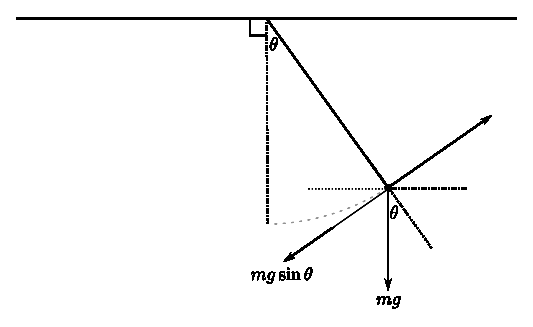
\includegraphics[scale=1.0]{img/pendulum}
\caption{Sketch of a pendulum of length $l$ with a mass $m$, displaying the forces acting on the mass resolved in the tangential direction relative to the motion. }
\end{figure}

Using Newton's second law of motion $F=ma$, we have the differential equation:
\[-mg\sin\theta=ml\ddot{\theta}\]

We re-write the equation as 
\[\ddot{\theta}+\frac{g}{l}\sin\theta=0.\]
This is a nonlinear equation, and we can not solve it analytically. 

When $\theta$ is small, $\sin\theta\approx\theta$ and so:
\[\ddot{\theta}+\omega^2\theta=0,\quad \omega=\sqrt{\frac{g}{l}}.\]

This is the equation for simple harmonic motion which we gave above. We can now solve this equation.

The auxilliary equation is

\begin{align*}
\lambda^2+\omega^2&=0\\
\lambda^2&=-\omega^2\\
\lambda&=\pm\omega\sqrt{-1}
\end{align*}

Therefore the solution of the ODE is:

\[\theta(t)=A\cos\omega t + B\sin\omega t.\]

\hrule
\vspace{2mm}

If the pendulum is displaced by an angle $\theta_0$ and released, then $\theta(0)=\theta_0$ and $\dot{\theta}(0)=0$, so
\[\theta(0)=A=\theta_0, \quad \dot{\theta}(0)=B\omega=0 \quad \implies \quad B=0,\]
therefore 
\[\theta(t)=\theta_0\cos\omega t \quad\implies\quad |\theta(t)|\le \theta_0.\]
\end{example}

The example above claims that the object on the pendulum will continue to swing forever. In reality the pendulum will slow down due to air resistance.

In order for our pendulum to do this, we must add air resistance to the ODE.

\begin{example}[A pendulum with air resistance]
As the pendulum is swinging, it will be subject to air resistance. The force due to air resistance will be proportional to the speed of the pendulum.
This leads to the ODE \[\ddot\theta + c \dot\theta + \frac{g}{l}\theta = 0,\] where $c$ is a constant.
\end{example}

We have learnt enough about ODEs that we can solve this equation, although we're not going to.
